\section{Reproduction results}

Table~\ref{tab:results} and Figures~\ref{fig:main-results}--\ref{fig:training}
group the component study and the extensions. Rows in
the first block are controlled comparisons at the same budget. Extension rows
vary capacity, epochs or augmentation, so their differences are descriptive.
All numbers are single-seed point estimates; differences below about one point
should not be read as reliable.

\begin{table}[!ht]
\centering
\caption{Test-split results. Epochs are 40 unless the run label says otherwise. PSDS1 uses IoU-0.5 matching (PSDS1@0.5); published PSDS1 is not directly comparable. Collar-F1 uses threshold 0.5 for the first block and 0.3 for wide/XL/mixup; class-wise rows use per-class thresholds.}
\label{tab:results}
\begin{tabular}{lcccc}
\toprule
Run & PSDS1@0.5 & PSDS2 & collar-F1 & frame-F1 \\
\midrule
BL: frame BCE + median & 36.67 & 73.13 & 26.11 & 59.14 \\
+RED & 37.16 & 71.43 & 26.47 & 59.01 \\
+OOL & 35.93 & 71.26 & 26.57 & 57.85 \\
+EPN, $\lambda_{\mathrm{iou}}=2$ & 25.87 & 51.41 & 13.57 & 35.95 \\
+EPN, $\lambda_{\mathrm{iou}}=1.0$ & 33.08 & 66.13 & 20.13 & 50.33 \\
+EPN, $\lambda_{\mathrm{iou}}=0.5$ & 35.42 & 69.83 & 21.39 & 55.17 \\
Wide model, 40 ep & 43.58 & 73.73 & 28.12 & 62.30 \\
Wide model, 100 ep & 44.28 & 70.77 & 31.50 & 63.16 \\
Wide, OOL=10, 60 ep & 42.97 & 72.62 & 28.87 & 61.47 \\
XL model, 60 ep & 45.02 & 72.38 & 31.98 & 63.56 \\
Synthetic mixup, $p=0.5$, 40 ep & 34.22 & 67.80 & 20.99 & 52.89 \\
Wide + mild mixup, 60 ep & 45.77 & 76.11 & 30.63 & 64.06 \\
XL + class-wise MF & 44.05 & 73.28 & 32.16 & 63.56 \\
Ensemble: XL + Wide + OOL10 & 46.81 & 75.17 & 30.77 & -- \\
Ensemble: four models & \textbf{47.73} & \textbf{76.74} & 30.99 & -- \\
\bottomrule
\end{tabular}
\end{table}

\begin{figure}[t]
\centering
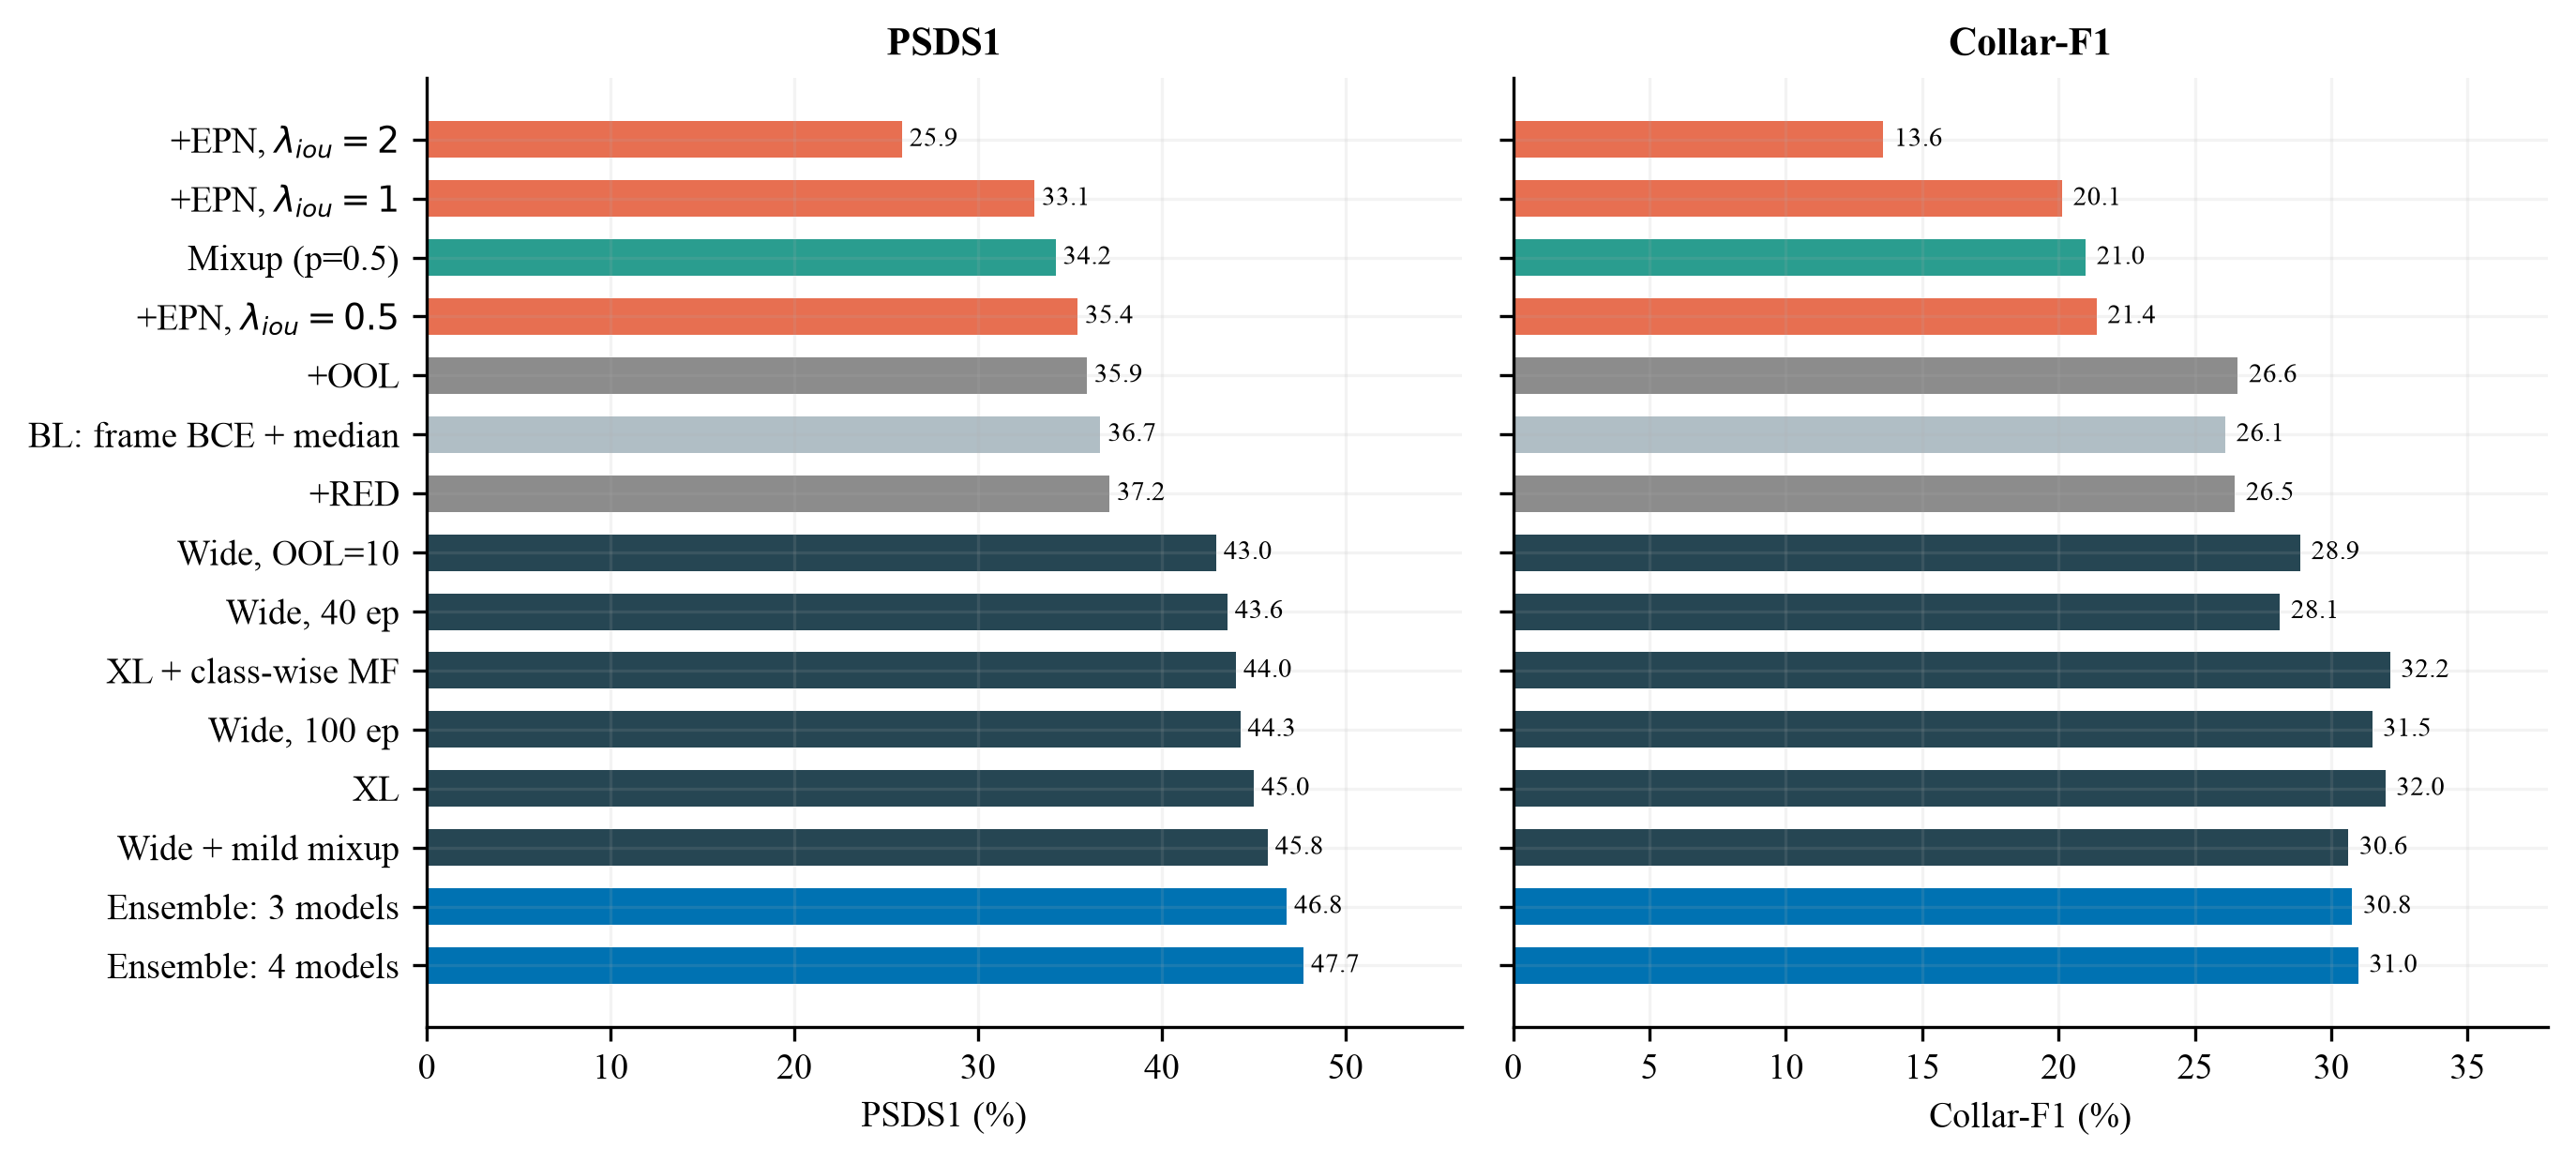
\includegraphics[width=\linewidth]{figures/fig_main_comparison.png}
\caption{Test PSDS1 and collar-F1 for the component study and the two
extensions and the post-processing variants. Red bars are full boundary-aware
runs, grey bars are frame-level or RED-only variants, teal bars are mixup runs,
dark blue bars are the wider/XL family, and light blue bars are ensembles.}
\label{fig:main-results}
\end{figure}

\begin{figure}[t]
\centering
\begin{minipage}{0.48\linewidth}
  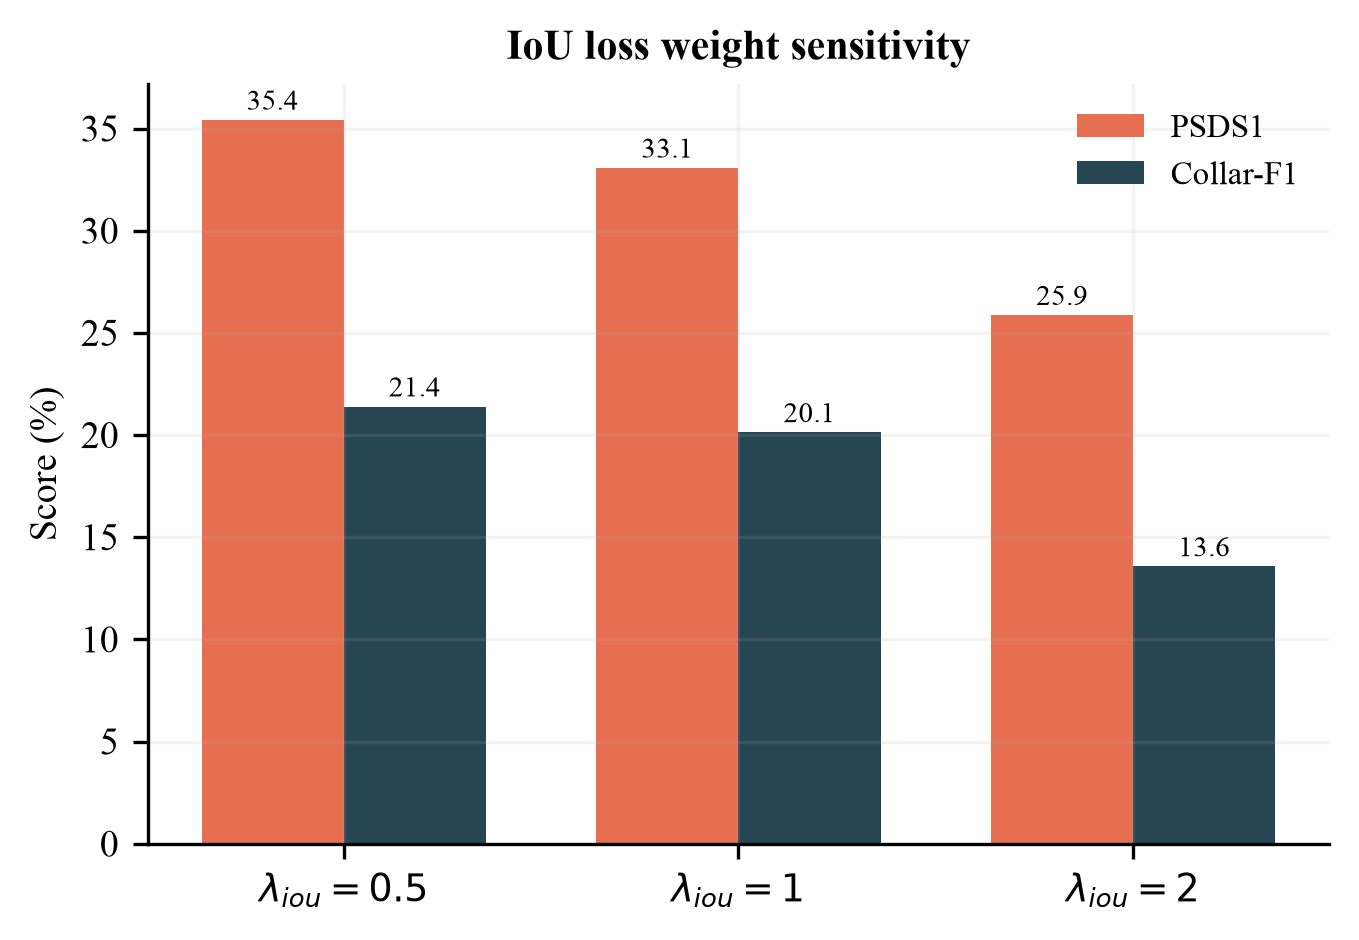
\includegraphics[width=\linewidth]{figures/fig_iou_sweep.png}
\end{minipage}\hfill
\begin{minipage}{0.48\linewidth}
  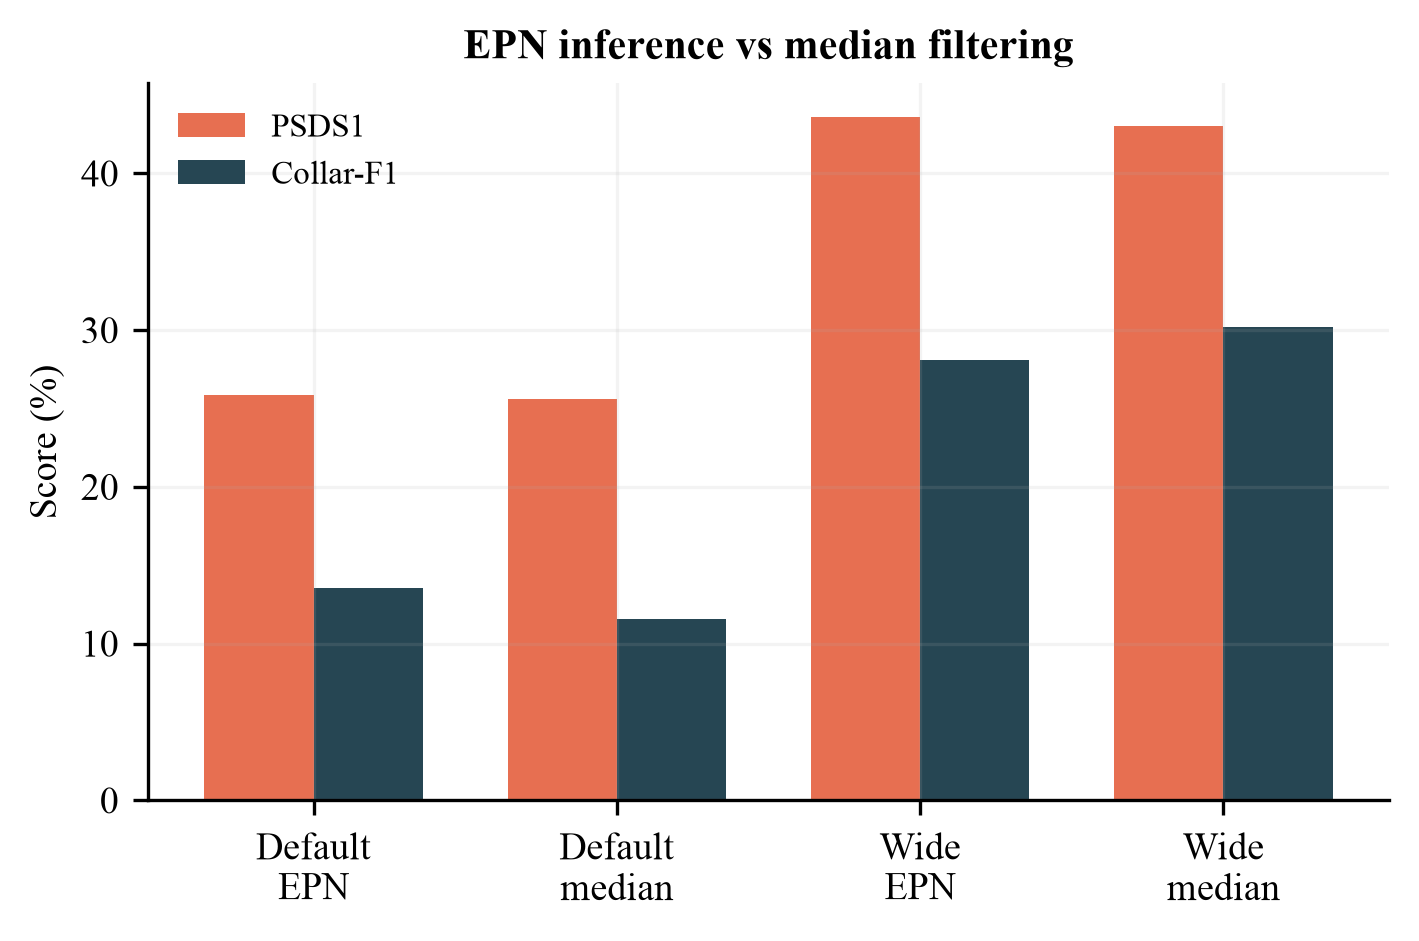
\includegraphics[width=\linewidth]{figures/fig_postprocessing.png}
\end{minipage}
\caption{Left: PSDS1@IoU0.5 and collar-F1 against the IoU loss weight. Right:
EPN inference against a validation-tuned median filter for the default and wide
models.}
\label{fig:iou-post}
\end{figure}

\begin{figure}[t]
\centering
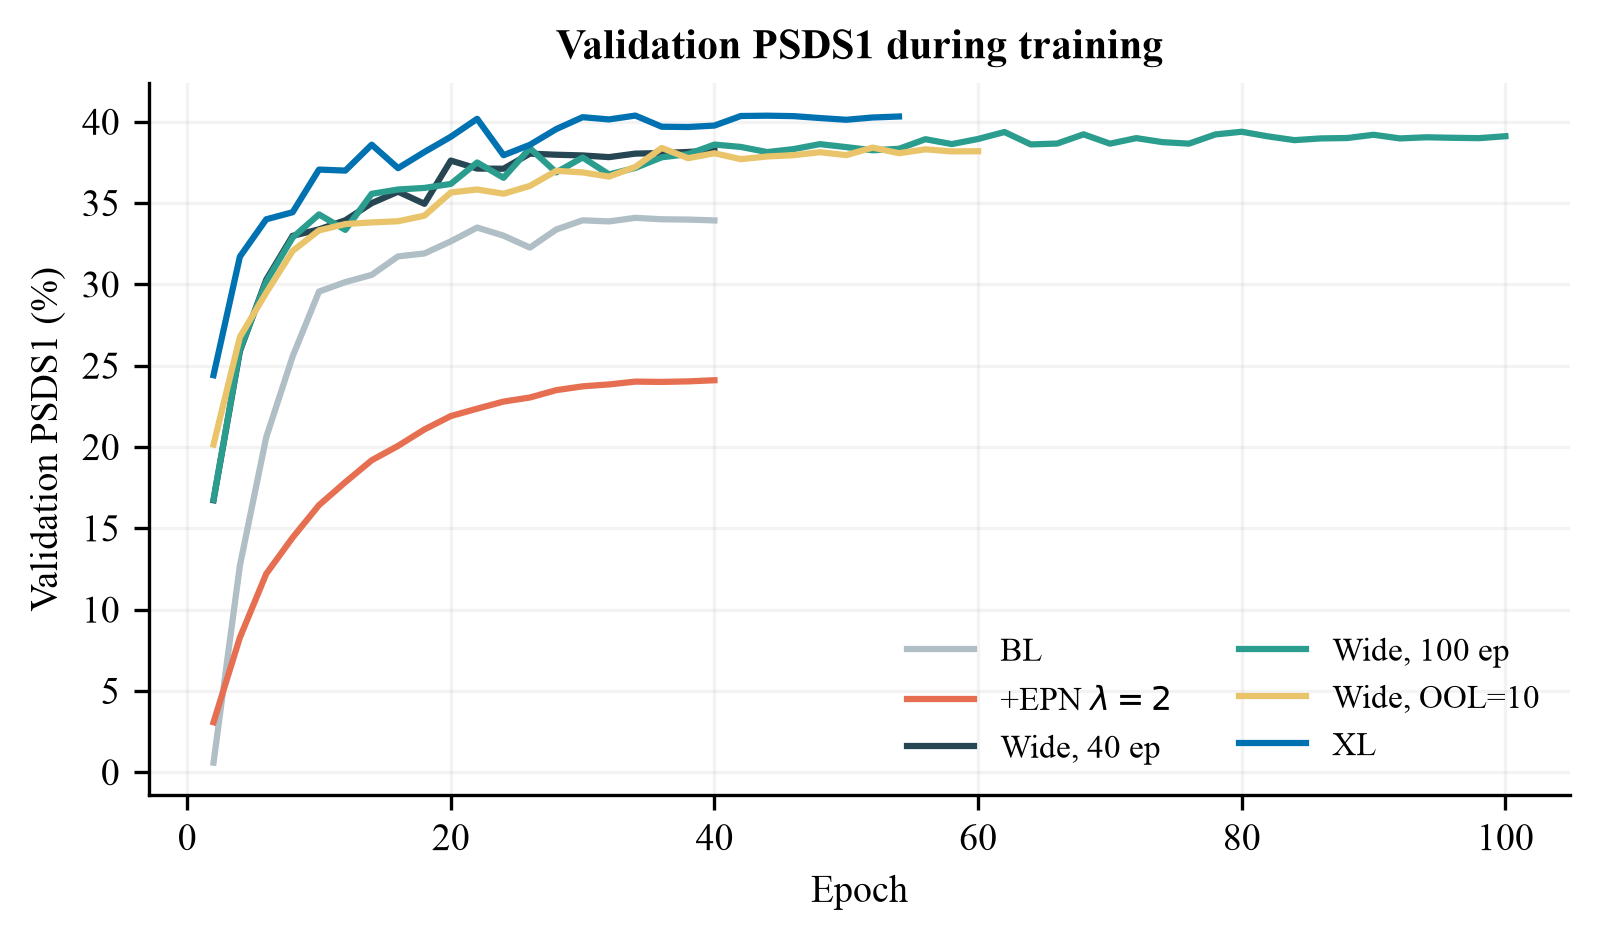
\includegraphics[width=0.78\linewidth]{figures/fig_training_curves.png}
\caption{Validation PSDS1@IoU0.5 during training. The wide-100 run continues to
improve after 40 epochs; the XL run is nearly flat after epoch 35; the default
model with $\lambda_{\mathrm{iou}}=2$ plateaus early.}
\label{fig:training}
\end{figure}

Main observations:
\begin{itemize}
\item RED alone is within 0.5 PSDS1 of the baseline (37.16 vs 36.67). With one
      seed this difference is not resolvable, so the result is consistent with
      the recurrence being neutral rather than harmful.
\item OOL at $\lambda_{\mathrm{ool}}=100$ does not help on URBAN-SED (35.93).
\item The IoU weight matters: $\lambda_{\mathrm{iou}}=2$ gives 25.87,
      $\lambda_{\mathrm{iou}}=1$ gives 33.08, and $\lambda_{\mathrm{iou}}=0.5$
      gives 35.42.
\item Capacity and training length help: the wide model reaches 43.58 at 40
      epochs, 44.28 at 100 epochs, and the XL model reaches 45.02.
\item Lowering OOL to 10 does not improve the wide model (42.97), so the
      boundary loss is not the limiting factor here.
\item Max-mix augmentation at $p=0.5$ hurts (34.22), but that run uses the
      default backbone while the mild $p=0.2$ run uses the wide backbone; the
      two are not a controlled mixing-probability sweep. The mild run reaches
      45.77 PSDS1 and 76.11 PSDS2.
\item Class-wise median tuning gives 44.05 PSDS1 and 32.16 collar-F1 on the XL
      model. It improves collar-F1 but not PSDS1.
\item Mild mixup reaches 45.77 PSDS1 and 76.11 PSDS2, the best single model.
\item A four-model probability ensemble reaches \textbf{47.73 PSDS1} and
      76.74 PSDS2. The members were selected after inspecting test scores, so
      this is an optimistic estimate; it is not a blind model-selection result.
\end{itemize}

\begin{table}[!ht]
\centering
\caption{Source-paper PSDS1 (AS-Strong-10, CRNN) next to the closest
reproduction rows. The datasets differ, so the columns are not directly
comparable; the table makes the reproduction gap explicit.}
\label{tab:source}
\begin{tabular}{lcc}
\toprule
Configuration & Paper (AS-Strong-10) & Reproduction (URBAN-SED) \\
\midrule
BL & 41.1 & 36.67 \\
+RED & 42.9 & 37.16 \\
+OOL & 46.2 & 35.93 \\
+EPN & 48.0 & 35.42 ($\lambda_{\mathrm{iou}}=0.5$; 25.87 at 2.0) \\
\bottomrule
\end{tabular}
\end{table}

\paragraph{Reproduction verdict.}
The paper's component ordering did not reproduce on URBAN-SED. At the paper's
default $\lambda_{\mathrm{iou}}=2$, the full method falls below the frame-wise
baseline (25.87 vs 36.67 PSDS1). Lowering the weight to $0.5$ recovers most of
the loss (35.42) but still does not beat the baseline. A tuned median filter on
the same wide model is essentially tied with EPN inference (43.00 vs 43.58
PSDS1), so the evidence here does not show that learned proposals remove the
need for post-processing. The improvements that do hold are capacity, longer
training, mild augmentation and probability ensembling. These are negative
reproduction findings about this dataset and budget, not a claim that the method
cannot work on AudioSet Strong.

